%
% The first command in your LaTeX source must be the \documentclass command.
\documentclass[acmlarge,screen]{acmart}
\usepackage{wrapfig}
\usepackage{tikz}
\def\BibTeX{{\rm B\kern-.05em{\sc i\kern-.025em b}\kern-.08emT\kern-.1667em\lower.7ex\hbox{E}\kern-.125emX}}
\begin{document}

%
% The "title" command has an optional parameter, allowing the author to define a "short title" to be used in page headers.
\title{Tarea No. 4. Procesamiento de Grafos}

%
% The "author" command and its associated commands are used to define the authors and their affiliations.
% Of note is the shared affiliation of the first two authors, and the "authornote" and "authornotemark" commands
% used to denote shared contribution to the research.

\author{Sebastian Gonzalo Vives Faus}
\affiliation{%
  \institution{Tecnológico de Monterrey}
}

% Logo del Tec en la derecha superior, usando el paquete de `tikz'
\begin{tikzpicture}[remember picture,overlay]
    \node[anchor=north east,yshift=-1.5pt,xshift=1pt]%
        at (current page.north east)
        {
\includegraphics[scale = 0.2]{tec}};
    \end{tikzpicture}


%
% The abstract is a short summary of the work to be presented in the article.
\begin{abstract}
El alumno aprenderá a trabajar con conjuntos de datos disponibles públicamente y a procesarlos utilizando alguna biblioteca ya existente para la programación de grafos así como visualizarlos con herramientas gráficas para descubrir información relevante. Adicionalmente, aprenderá a crear un artículo de investigación en formato de la ACM utilizando LaTEX.
\end{abstract}


\maketitle

\section{Introducción}
Esta investigación tiene como objetivo demostrar paso a paso como importar un dataset (dirigido), de la base de datos de SNAP \cite{SNAPdata}, a un grafo, utilizando C++. Con el grafo obtenido, exportarlo con cuatro funciones, las cuales exportaran el grafo en los siguientes formatos: GraphML, GEXF, GDF y JSON Graph Format. Se obtendrá el tiempo de ejecución que le toma a cada función exportar el grafo en su determinado formato. Una vez exportado los grafos, se utiliza un programa llamado Gephi, para la visualización de uno de los grafos (en este caso, se elegio el formato GraphML). Se obtendrá una imagen, representando el grafo. Finalmente, se utilizará LaTEX (con el template ACM) para demostrar y explicar los resultados obtenidos.

\section{Procesamiento en C++}

\subsection{Importación}
Lo primero que se hizo fue importar un data set de la base de datos de SNAP (en este caso, en la sección de {\it Large Network Dataset Collection}) [1]. El data-set obtenido para este ejemplo fue el de las votaciones de Wikipedia, desde que se creó hasta el 2008. Este data-set contiene un total de {\it 7115 Nodos} y {\it 103,689 Vértices}.\\ \\ Una vez obtenido el data set (archivo .txt), vamos a nuestro código de C++. Utilizamos la función de importar el data set a un grafo (obtenido de la Documentación de SNAP) \cite{SNAPdev}:
\\ \\
\textbf{ PGraph TSnap::LoadEdgeList( const TStr InFNm, const int SRCColld, const int DstColld )}

\pagebreak

\begin{verbatim}
TSsParser Ss("Wiki-Vote.txt", ssfWhiteSep, true, true, true); 
int SrcNId, DstNId, SrcColId = 0, DstColId = 1;

while (Ss.Next()) {
       if (! Ss.GetInt(SrcColId, SrcNId) || ! Ss.GetInt(DstColId, DstNId)) { continue; }
       if (! Graph->IsNode(SrcNId)) { Graph->AddNode(SrcNId); }
       if (! Graph->IsNode(DstNId)) { Graph->AddNode(DstNId); }
       Graph->AddEdge(SrcNId, DstNId);
      }
       Graph->Defrag();

\end{verbatim}
Donde tenemos que proporcionarle el {\it archivo del data set}, al igual que las columnas donde se encuentran el {\it nodo origen} (SrcColId) y el {\it nodo destino} (DstColId). Una vez importado, podemos comprobar que la cantidad de nodos y vertices en el grafo coincida con lo indicado en el data set, utilizando la función de SNAP:
\\

\begin{verbatim}
  void PrintGStats(const char s[], PNEGraph Graph) {
  printf(" %s nodos %d, edges %d, esta vacia? = %s\n",
      s, Graph->GetNodes(), Graph->GetEdges(),
      Graph->Empty() ? "Si" : "No");
  }
\end{verbatim}

\subsection{Exportación}
Ahora que tenemos toda la información del grafo dentro de nuestro programa, podemos empezar a hacer el proceso de {\it exportación}. El grafo será exportado utilizando cuatro funciones \cite{git}, enseñadas a continuación:
\begin{itemize}
\item GraphML \label{GraphML}
 \begin{verbatim}
 void GraphML(PNEGraph Graph) {
	//Variables
	ofstream file ("Wiki-Vote.graphml"); //Archivo de salida
	int i = 1;
	//GraphML:
	if (file.is_open()) {
		file << "<?xml version=\"1.0\" encoding=\"UTF-8\"?>\n";
		file << "<graphml xmlns=\"http://graphml.graphdrawing.org/xmlns\" xmlns:xsi=
		\"http://www.w3.org/2001/XMLSchema-instance\" xsi:schemaLocation=
		\"http://graphml.graphdrawing.org/xmlns http://graphml.graphdrawing.org/xmlns/1.0/graphml.xsd\">\n";
		file << "<graph id=\"G\" edgedefault=\"directed\">\n";

		for (PNEGraph::TObj::TNodeI NI = Graph->BegNI(); NI < Graph->EndNI(); NI++){
			file << "<node id=\"" << NI.GetId() << "\"/>\n";
		}

		for (PNEGraph::TObj::TEdgeI EI = Graph->BegEI(); EI < Graph->EndEI(); EI++, ++i){
			file << "<edge id=\"e" << i << "\" source=\"" << EI.GetSrcNId() << "\" target=\"" <<
			 EI.GetDstNId() << "\"/>\n";
		}

		file << "</graph>\n";
		file << "</graphml>\n";
		file.close();
	}
}
 \end{verbatim}
\item GEXF \label{GEXF}
 \begin{verbatim}
  void GEXF(PNEGraph Graph) {
	//Variables
	ofstream file ("Wiki-Vote.gexf"); //Archivo de salida
	int i = 1;
	//GEXF:
	if (file.is_open()) {
		file << "<?xml version=\"1.0\" encoding=\"UTF-8\"?>\n";
		file << "<gexf xmlns=\"http://www.gexf.net/1.2draft\" version=\"1.2\">\n";
		file << "<graph mode=\"static\" defaultedgetype=\"directed\">\n";
		file << "<nodes>\n";

		for (PNEGraph::TObj::TNodeI NI = Graph->BegNI(); NI < Graph->EndNI(); NI++){
			file << "<node id=\"" << NI.GetId() << "\" />\n";
		}

		file << "</nodes>\n";
		file << "<edges>\n";

	for (PNEGraph::TObj::TEdgeI EI = Graph->BegEI(); EI < Graph->EndEI(); EI++, ++i){
		file << "<edge id=\"" << i << "\" source=\"" << EI.GetSrcNId() << "\" target=\"" <<
		 EI.GetDstNId() << "\" />\n";
	}

		file << "</edges>\n";
		file << "</graph>\n";
		file << "</gexf>\n";
		file.close();
	}
}
 \end{verbatim}
 
 \item GDF  \label{GDF}
 \begin{verbatim}
  void GDF(PNEGraph Graph) {
	ofstream file ("Wiki-Vote.gdf"); //Archivo de salida
	//GDF:
	if (file.is_open()) {
		file << "nodedef>id VARCHAR\n";
		for (PNEGraph::TObj::TNodeI NI = Graph->BegNI(); NI < Graph->EndNI(); NI++){
			file << NI.GetId() << "\n";
		}

		file << "edgedef>source VARCHAR, destination VARCHAR\n";
		for (PNEGraph::TObj::TEdgeI EI = Graph->BegEI(); EI < Graph->EndEI(); EI++){
			file << EI.GetSrcNId() << ", " << EI.GetDstNId() << "\n";
		}

		file.close();
	}
}
 \end{verbatim}
 
 \item JSON  \label{JSON}
 \begin{verbatim}
  void JSON(PNEGraph Graph) {
	ofstream file ("Wiki-Vote.json"); //Archivo de salida
	if (file.is_open()) {
		file << "{ \"graph\": {\n";
		file << "\"nodes\": [\n";
		for (PNEGraph::TObj::TNodeI NI = Graph->BegNI(); NI < Graph->EndNI(); ){
			file << "{ \"id\": \"" << NI.GetId() << "\" }";
			if (NI++ == Graph->EndNI())
				file << " ],\n";
			else
				file << ",\n";
		}

		file << "\"edges\": [\n";
		for (PNEGraph::TObj::TEdgeI EI = Graph->BegEI(); EI < Graph->EndEI(); ){
			file << "{ \"source\": \"" << EI.GetSrcNId() << "\", \"target\": \"" << EI.GetDstNId() << "\" }";
			if (EI++ == Graph->EndEI())
				file << " ]\n";
			else
				file << ",\n";
		}
		file << "} }";

		file.close();
	}
}
 \end{verbatim}

\end{itemize}

Cada función genera su propio archivo de salida ({\it .graphml, .gexf, .gdf, .json}), los cualaes pueden ser utilizados en otros programas de graficación de grafos (en nuestro caso, este será {\it Gephi}).

\subsection{Tiempo de Ejecución}
Como parte de esta investigación, es requerido calcular el {\it tiempo de ejecución} de cada función de exportación, con el fin de comparar cada tiempo y determinar cuál de las cuatro funciones es la más rápida. Para encontrar el tiempo de ejecución de cada función (en {\it milisegundos} ), se utilizaron las siguientes funciones:
\\
\begin{verbatim}
    //Variables de tiempo;
    high_resolution_clock::time_point start;
    high_resolution_clock::time_point finish;
    
    //Empieza el tiempo
    start = high_resolution_clock::now();
    
    //Termina el tiempo
    finish = high_resolution_clock::now();
    
    //Obten la duración restando el tiempo final - tiempo inicial
    auto duration = std::chrono::duration_cast<std::chrono::milliseconds>( finish - start ).count();

\end{verbatim}

Los resultados (probando el código cinco veces y obteniendo el tiempo promedio de cada uno) de las funciones se pueden ver reflejados en la {\bf Tabla} ~\ref{tab:tiempos}.

\begin{table*}
 \caption{Resultados de lo Tiempos de Ejecución de las Funciones de Exportación}
 \label{tab:tiempos}
 \begin{tabular}{c|c|c|c|c|c}
  \toprule
  N. de Intento & T. de Importación ({\it ms})& GraphML ({\it ms})& GEXF ({\it ms})& GDF ({\it ms})& JSON ({\it ms})\\
  \midrule
  1 &49 & 138 & 138 & 33 & 54\\
  2	&67	&182	&152	&33	&56\\
  3	&44	&152	&158	&46	&66\\
  4	&54	&167	&150	&38	&79\\
  5	&43	&144	&186	&53	&88\\
  \bottomrule
  {\bf \it Promedio} & {\bf \it 51.4} & {\bf \it 156.6} & {\bf \it 156.8} & {\bf \it 40.6} & {\bf \it 68.6}
 \end{tabular}
\end{table*}

\section{Complejidad Temporal}
Los cuatro algoritmos comparten comparten la misma complejidad temporal en el mejor y caso promedio (no hay peor caso, ya que sería el mismo que el promedio). En el mejor caso (donde no entra el {\it if}, lo que significaría que el archivo de salida no estuvisese abierto por alguna razón externa) la complejidad del algoritmo es {\it O(1)}. En el caso promedio (hay dos {\it for}, pero ninguno dentro del otro) la complejidad del algoritomo es {\it $\Omega$(n)}.

\section{Análisis del grafo en Gephi}
Se analizó el grafo exportado por nuestro programa en C++ específicamente la extensión {\it .gexf}, ya que es el más compatible con Gephi (solo requerimos analizar solo uno de los cuatro métodos de exportación). Dentro del programa de Gephi, seguimos las siguientes instrucciones para importar el grafo dentro del programa:

\begin{enumerate}
 \item Abrir el programa de {\it Gephi} (versión actual: 0.9.2).
 \item En la ventana de inicio ({\it Welcome to Gephi}), ir a la opción: {\it Open graph file...} en la sección de {\it New Project}.
 \item Seleccionar el archivo exportado con extensión {\it .gexf}.
 \item Aparecerá una ventana de {\it Importación}, donde nos muestra si el grafo es dirigido o no, al igual que su número de Nodos y Vértices que contiene. Si los datos son correctos, darle a la opción de {\it OK}.
 \item A continuación, nos aparecerá una visualización de nuestro grafo, donde cada nodo esta conectado respectivo destino (las líneas son los vértices). Dependiendo la cantidad de nodos y vértices (en este caso son 7,115 nodos y 103,689 vértices) será la complejidad de la visualización (entre mas conexiones, más difícil se vuelve de navegar y observar las conexiones.
 \item Se puede ver la representación del grafo utilizado ({\it Wiki-Vote.gexf}) en la siguiente imágen ~\ref{fig:gephi}.
 \item Gephi permite al usuario jugar con la gráfica con sus herramientas predeterminadas. Mencionando algunas:
 \begin{itemize}
  \item Puedes mover, seleccionar, incrementar y disminuir el tamaño de la visualización de la gráfica.
  \item {\bf Painter:} Te permite cambiar el color de las nodos, seleccionandolos con el {\it mouse izquierdo}.
  \item {\bf Sizer:} Te permite modificar el tamaño de uno o múltiples nodos.
  \item {\bf Brush:} Te permite cambiar el color de un nodo y todos los nodos alrededor del nodo pintado.
  \item {\bf Node Pencil:} Te permite añadir un nuevo nodo.
  \item {\bf Edge Pencil:} Te permite agregar un vértice entre dos nodos.
  \item {\bf Shortest Path:} Te permite saber cual es el camino más corto entre dos nodos.
  \item {\bf Heat Map:} Te permite colocar un mapa de color en un grupo de nodos. El color varía dependiendo el peso (en nuestro caso, no hya peso).
  \item {\bf Edit:} Te permite editar los atributos de un nodo.
  \item Tambien te permite cambiar los colores y propiedades del ambiente de la gráfica.
  \item Por último (entre las funciones que nos interesan), nos permite {\it exportar} la visualización del grafo en un formato de .gephi e formato de {\it imágen}.
 \end{itemize}
\end{enumerate}

\begin{figure}[h!]
 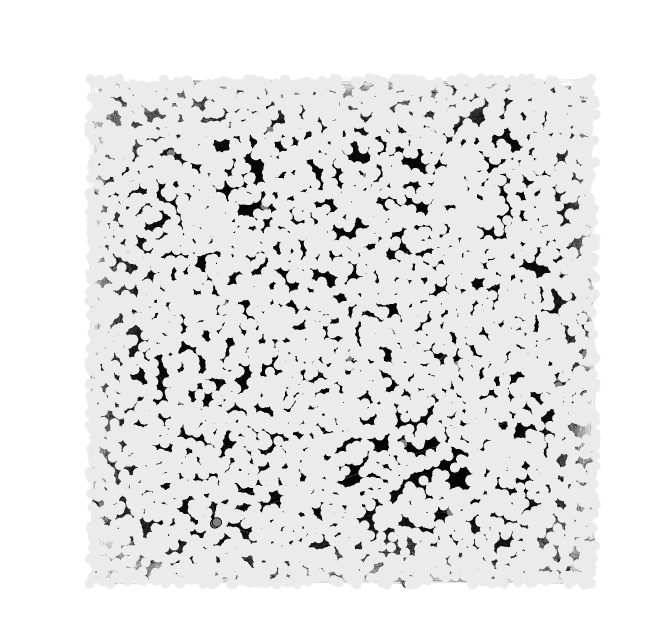
\includegraphics[scale=0.5]{Gephi_GML.png}
 \caption{Representación visual en Gephi}
 \label{fig:gephi}
\end{figure}

\begin{figure}[h!]
 
\includegraphics[scale=0.27]{GML_Imagen.png}
 \caption{Archivo de imágen (PNG) exportado de Gephi}
 \label{fig:gephiImg}
\end{figure}

\section{Ventajas y Desventajas}

\begin{itemize}
\item Una de las mayores desventajas del formato JSON es que no es soportado por Gephi, en comparación a los otros tres que sí son soportados. En términos de su tiempo de ejecución [\ref{tab:tiempos}], tuvo un promedio de {\it 68.6 ms}, poniendolo en el segundo más rápido en comparación a las otras funciones.
 \begin{figure}[h!]
 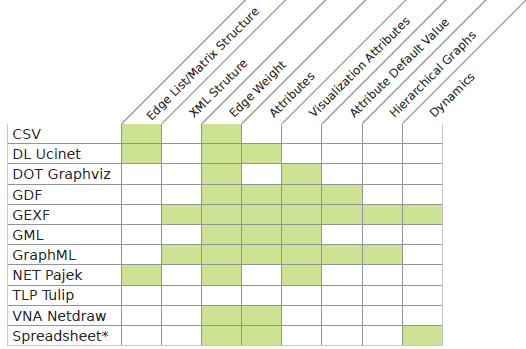
\includegraphics[scale=0.8]{graph-format-table-comparison.png}
 \caption{Tabla comparativa de las funcionalidades disponibles en Gephi de cada formato de grafo. Imagen obtenida de: Supported Graph Formats (\url{https://gephi.org/users/supported-graph-formats/})}
 \label{fig:gephitable}
 \end{figure}
 \item Ya que los otros tres formatos {\bf si} son soportados por Gephi, se muestra en la figura [\ref{fig:gephitable}] una tabla comparativa de todas las funciones disponibles para cada formato. Como se muestra en la tabla comparativa, la función con más funciones es GEXF, siguiendo GraphML y por último GDF. Por esa razón (entre otras), Gephi recomienda el uso del formato GEXF sobre cuaquier otro \cite{Gephi}. Tambien, el formato GEXF es el único que soporta el uso de pesos {\it dinamicos}. En términos de tiempos de ejecución [\ref{tab:tiempos}], fue el más que se tardó (promedio de {\it 68.6 ms})  en exportar el grafo (casi a la par con GraphML).
 \item Una de las ventajas de utilizar los formatos de GraphML, GEXF y GDF es que, son los únicos que formatos que pueden reconocer la posición de los nodos, su color y el tamaño de sus atributos.
\end{itemize}
\bibliographystyle{ACM-Reference-Format}
\bibliography{sample}

\section{URL Github}
\url{https://github.com/tec-csf/TC2017-T2-Otono-2019-Tlacuachi}

\end{document}
